\documentclass{beamer}
% \documentclass[notes]{beamer}
% \documentclass[notes=only]{beamer}
\usecolortheme{seahorse}

\title{AcCAPTCHA}
\author{Edoardo De Matteis}
\institute{Sapienza University of Rome}
\date{}

% * Commands

\begin{document}

\frame{\titlepage}

% \begin{frame}
% 	\frametitle{Table of Contents}
% 	\tableofcontents
% \end{frame}

% * Introduction
\begin{frame}
	\frametitle{Introduction}
	\emph{Completely Automated Public Turing test to tell Computers and Humans Apart.}

	\pause

	Any computer should be able to grade the test but not to pass it.

	\note[item]{Say the history of how CAPTCHAs became a thing in the Introduction's preamble.}
	\note[item]{We will now look at some historical background.}
\end{frame}

\begin{frame}
	\frametitle{CAPTCHA}
	The original idea is based on the fact that humans are extremely good at pattern and optical character recognition.
	\begin{figure}[h!t]
		\centering
		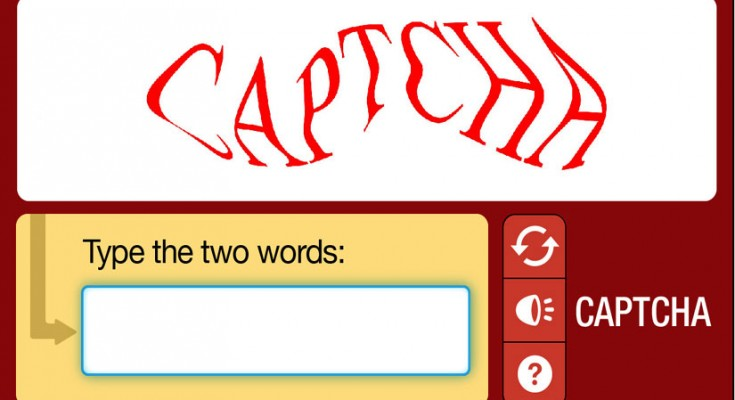
\includegraphics[scale=0.25]{assets/images/captcha.jpg}
	\end{figure}

	\note[item]{Brief history on CAPTCHA.}
\end{frame}

\begin{frame}
	\frametitle{reCAPTCHA}
	Implements a consensus based policy, with the machine not needing to know the second word.
	\begin{figure}[h!t]
		\centering
		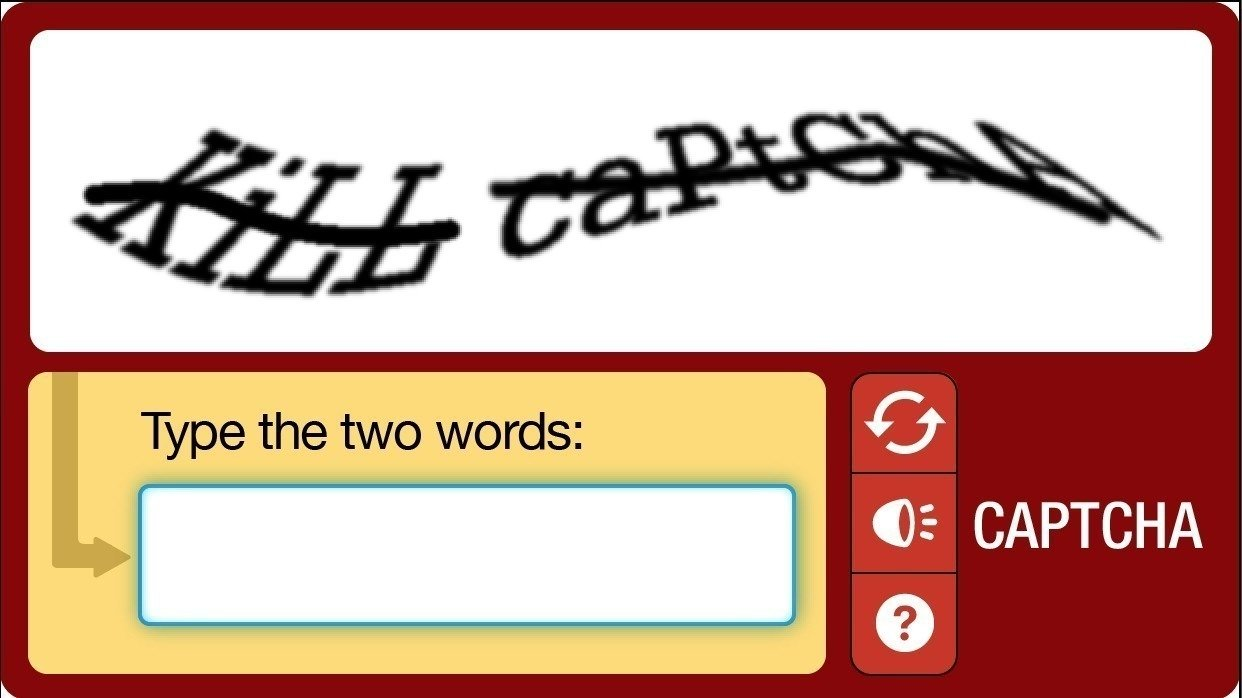
\includegraphics[scale=0.3]{assets/images/recaptcha.jpg}
	\end{figure}

	\note[item]{Brief history on reCAPTCHA.}
\end{frame}

\begin{frame}
	\frametitle{reCAPTCHAv2}
	Consensus-based, this time with images.
	\begin{figure}[h!t]
		\centering
		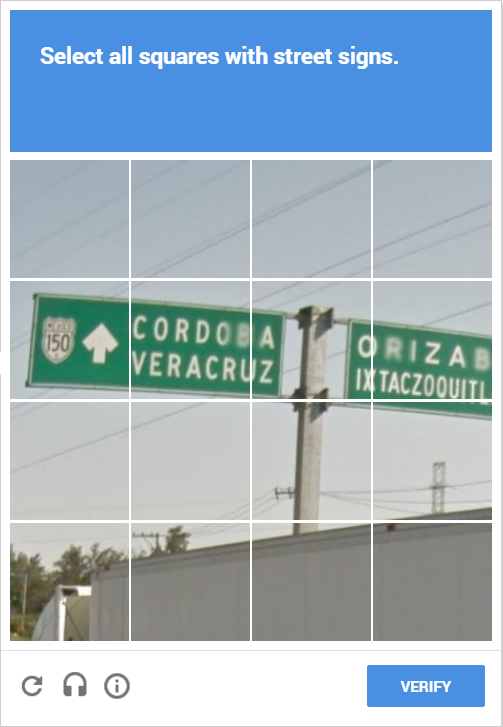
\includegraphics[scale=0.3]{assets/images/recaptchav2.png}
	\end{figure}

	\note[item]{Brief history on reCAPTCHAv2.}
\end{frame}

\begin{frame}
	\frametitle{NoCAPTCHA}
	Behavior-based and constantly running in the background.
	\begin{figure}[h!t]
		\centering
		
\includegraphics[scale=0.3]{assets/images/nocaptcha.jpg}
	\end{figure}

	\note[item]{Brief history on NoCAPTCHA.}
\end{frame}

\begin{frame}
	\frametitle{Methodology}
	The CAPTCHA problem is far from being solved and there are very few options for disabled people.

	AcCAPTCHA is a starting point for an accessible CAPTCHA system.

	\note[item]{It presents the following modalities}
	\note[item]{The user accesses the system through the web.}
	\note[item]{Aesthetically, you saw it. It is minimalistic and uses big characters for a reason.}
\end{frame}

\begin{frame}
	\frametitle{Text recognition}
	\begin{figure}[h!t]
		\centering
		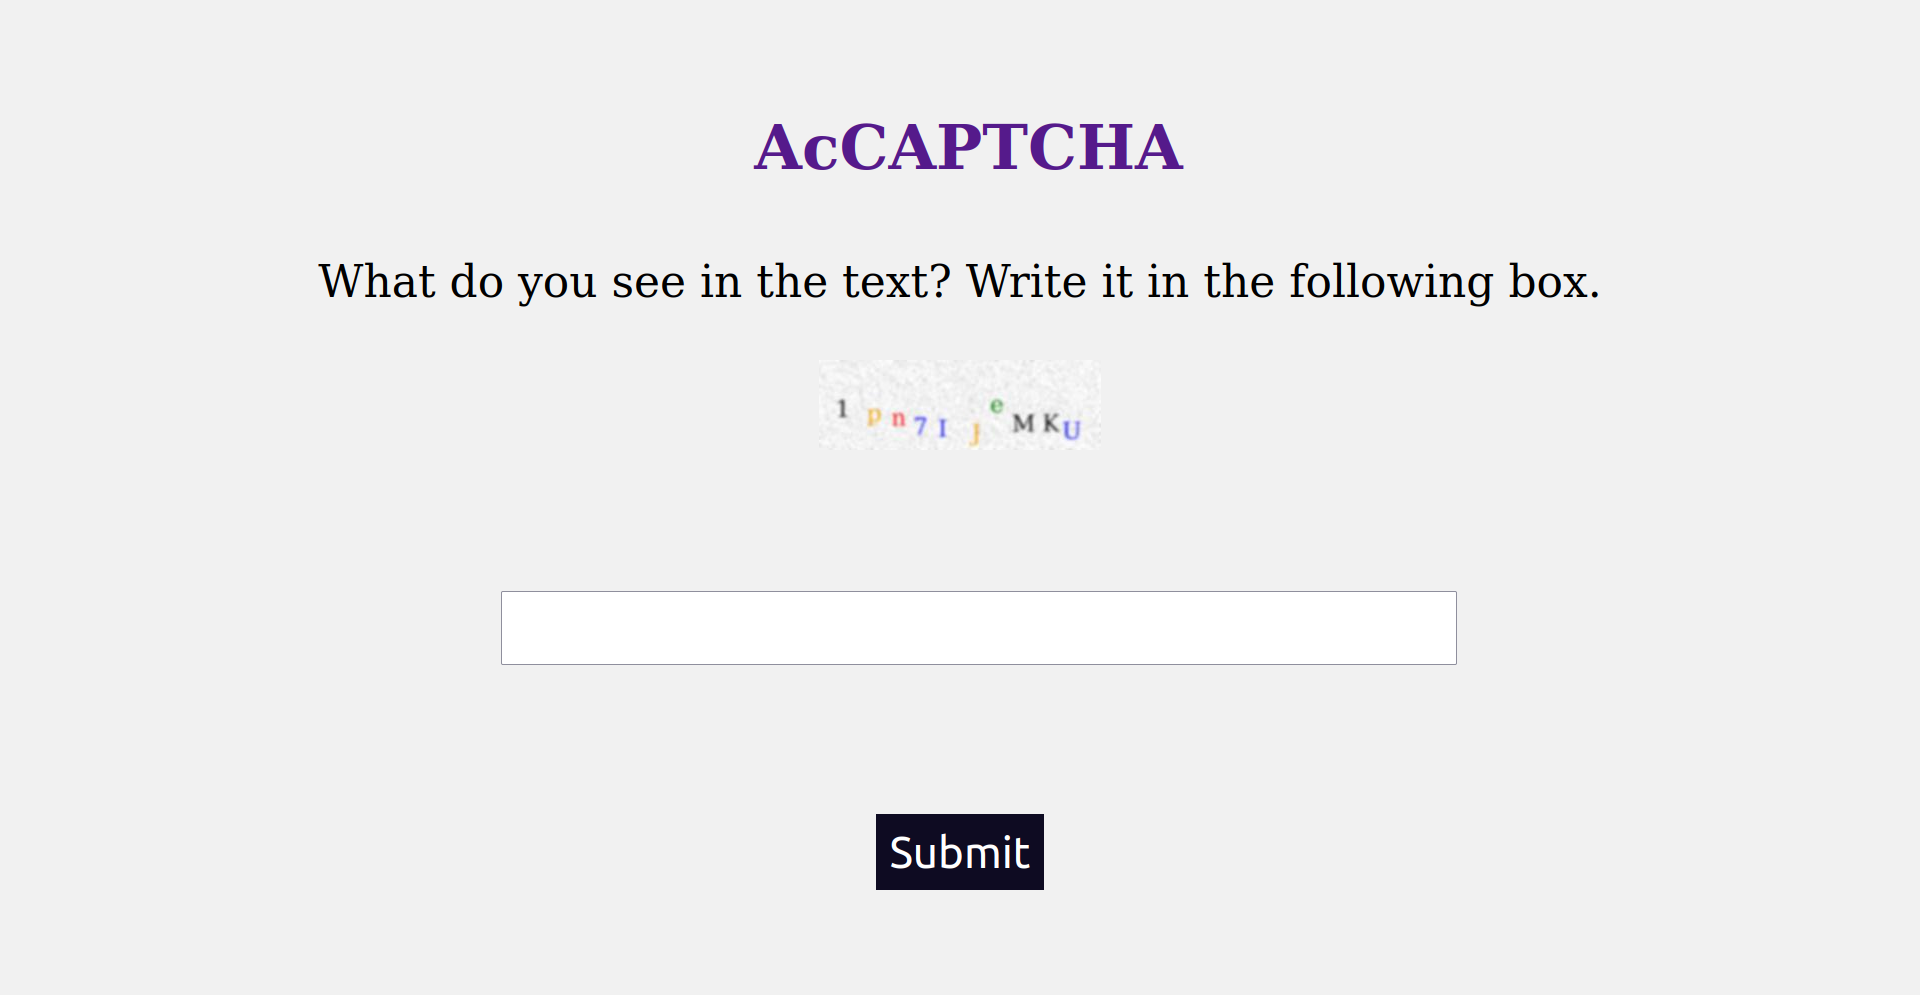
\includegraphics[scale=0.15]{assets/images/text_recognition.png}
	\end{figure}

\end{frame}
\begin{frame}
	\frametitle{Image classification}
	\begin{figure}[h!t]
		\centering
		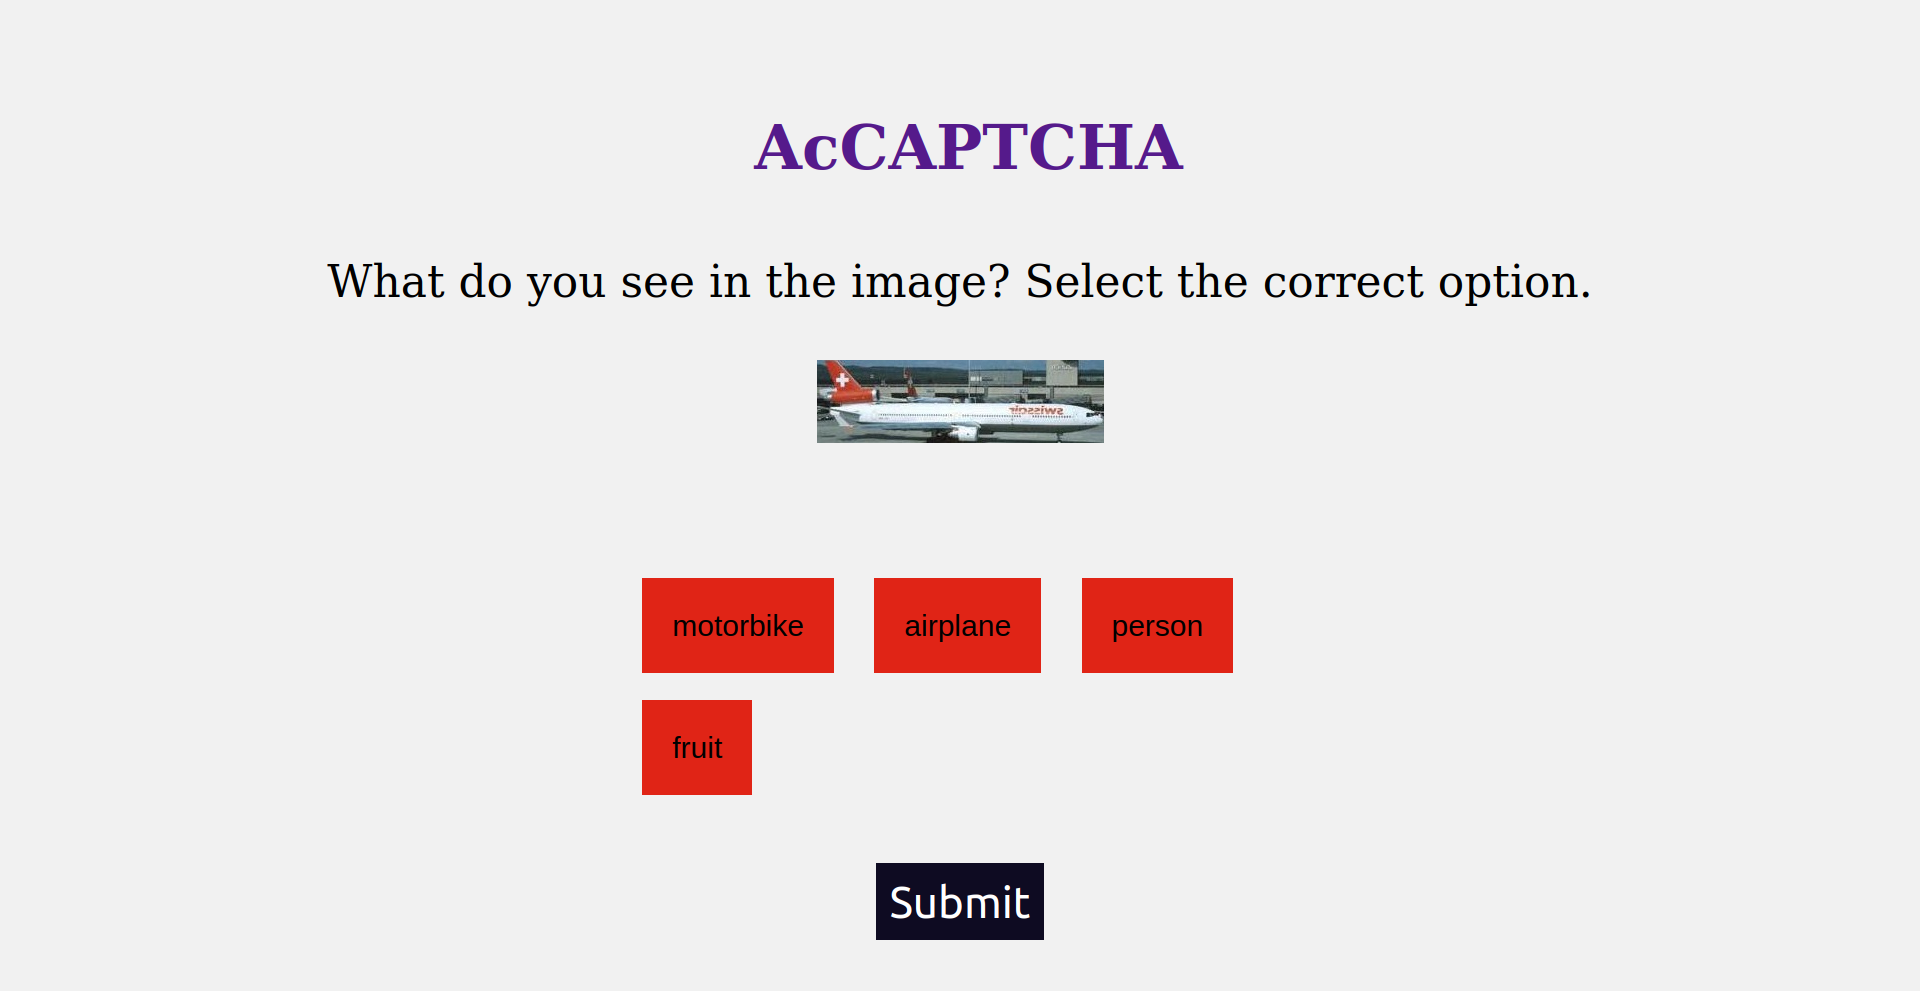
\includegraphics[scale=0.15]{assets/images/image_classification.png}
	\end{figure}

\end{frame}
\begin{frame}
	\frametitle{Finger counting}
	\only<1>{
		\begin{figure}[h!t]
			\centering
			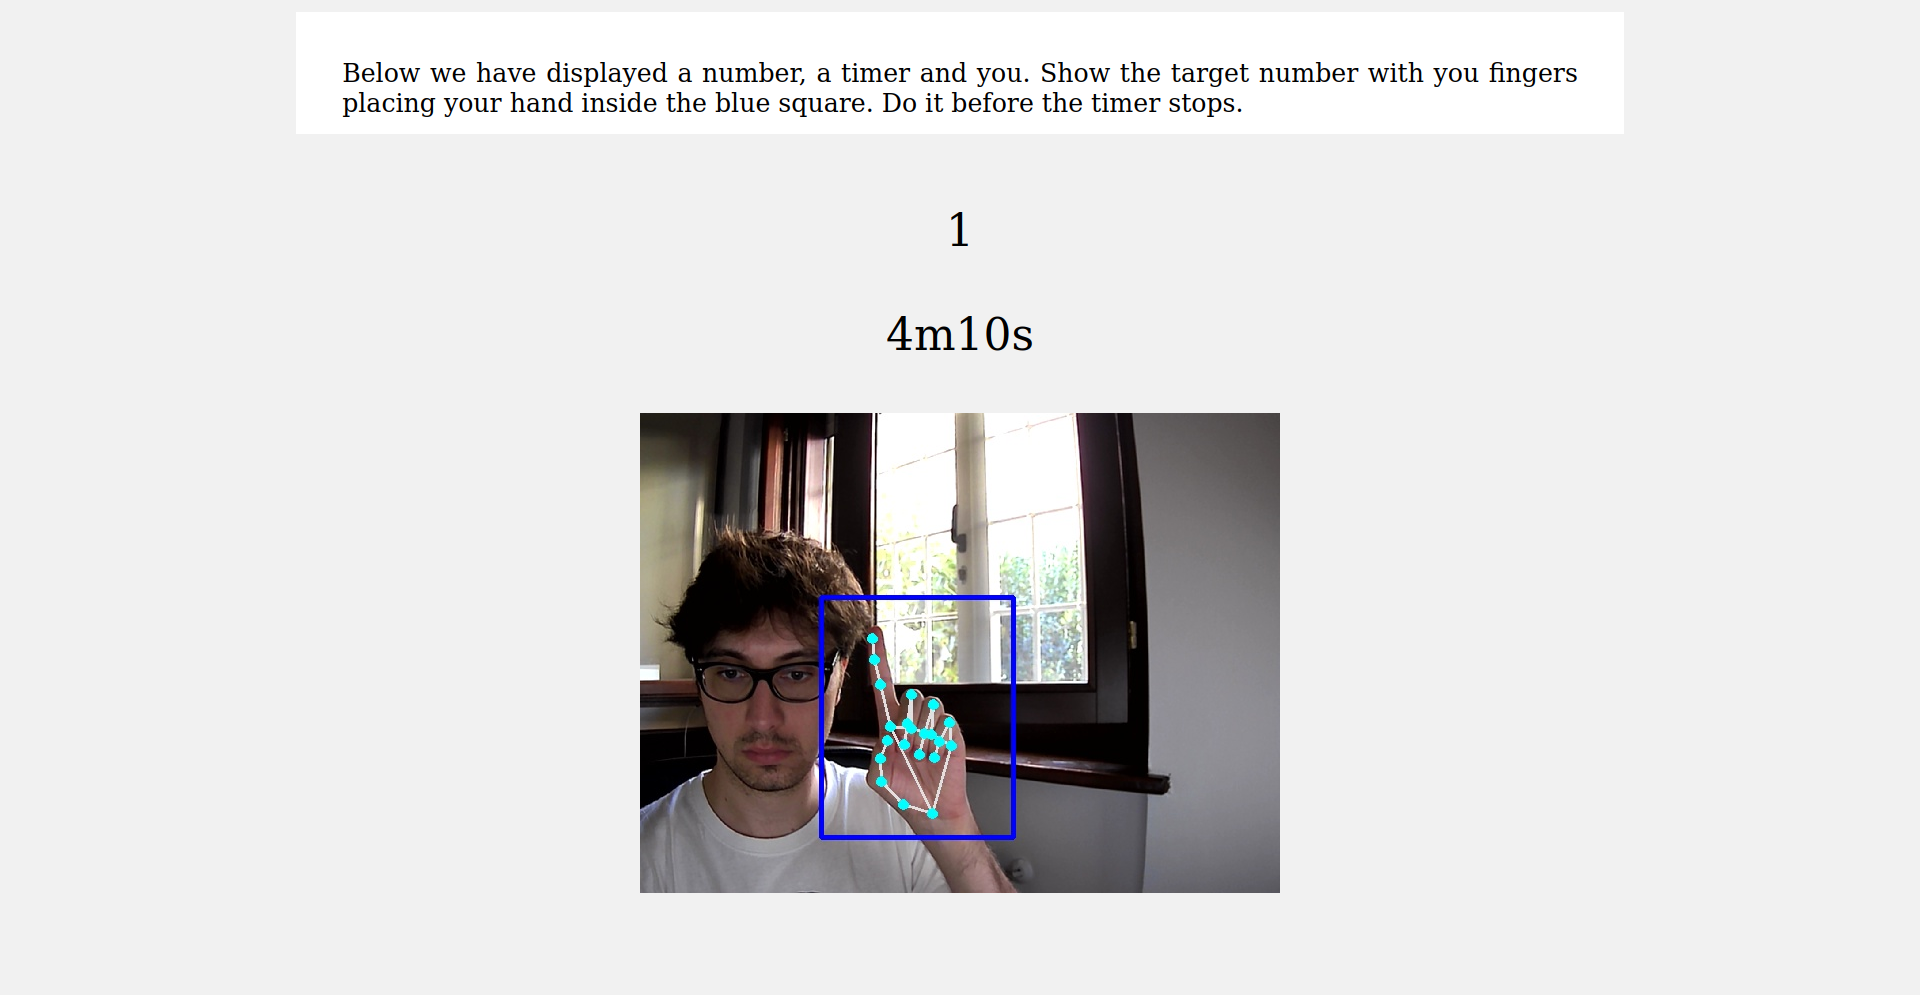
\includegraphics[scale=0.15]{assets/images/finger_count.png}
		\end{figure}
	}

	\begin{itemize}
		\item <2-> MMPOSE's hand recognition reaches 84\% AUC and 81\% PCK@0.2.
		\item <3-> Classic computer vision's issues.
		\item <4-> Cultural differences may or may not be a problem.
	\end{itemize}

	\note[item]<1>{The two previous tasks are too dependent on classic user abilites.}
	\note[item]<1>{Describe the input number, the counter and the RoI.}
	\note[item]<1>{It is a behavioral task.}
	\note[item]<2>{Describe what this model does.}
	\note[item]<2>{PCK@a is the Probability of Correct Keypoint at threshold a.}
	\note[item]<4>{Describe central Asia, Russia, chisanbop and european ways of counting.}
\end{frame}

\begin{frame}
	\frametitle{Word reading}
	\only<1>{
		\begin{figure}[h!t]
			\centering
			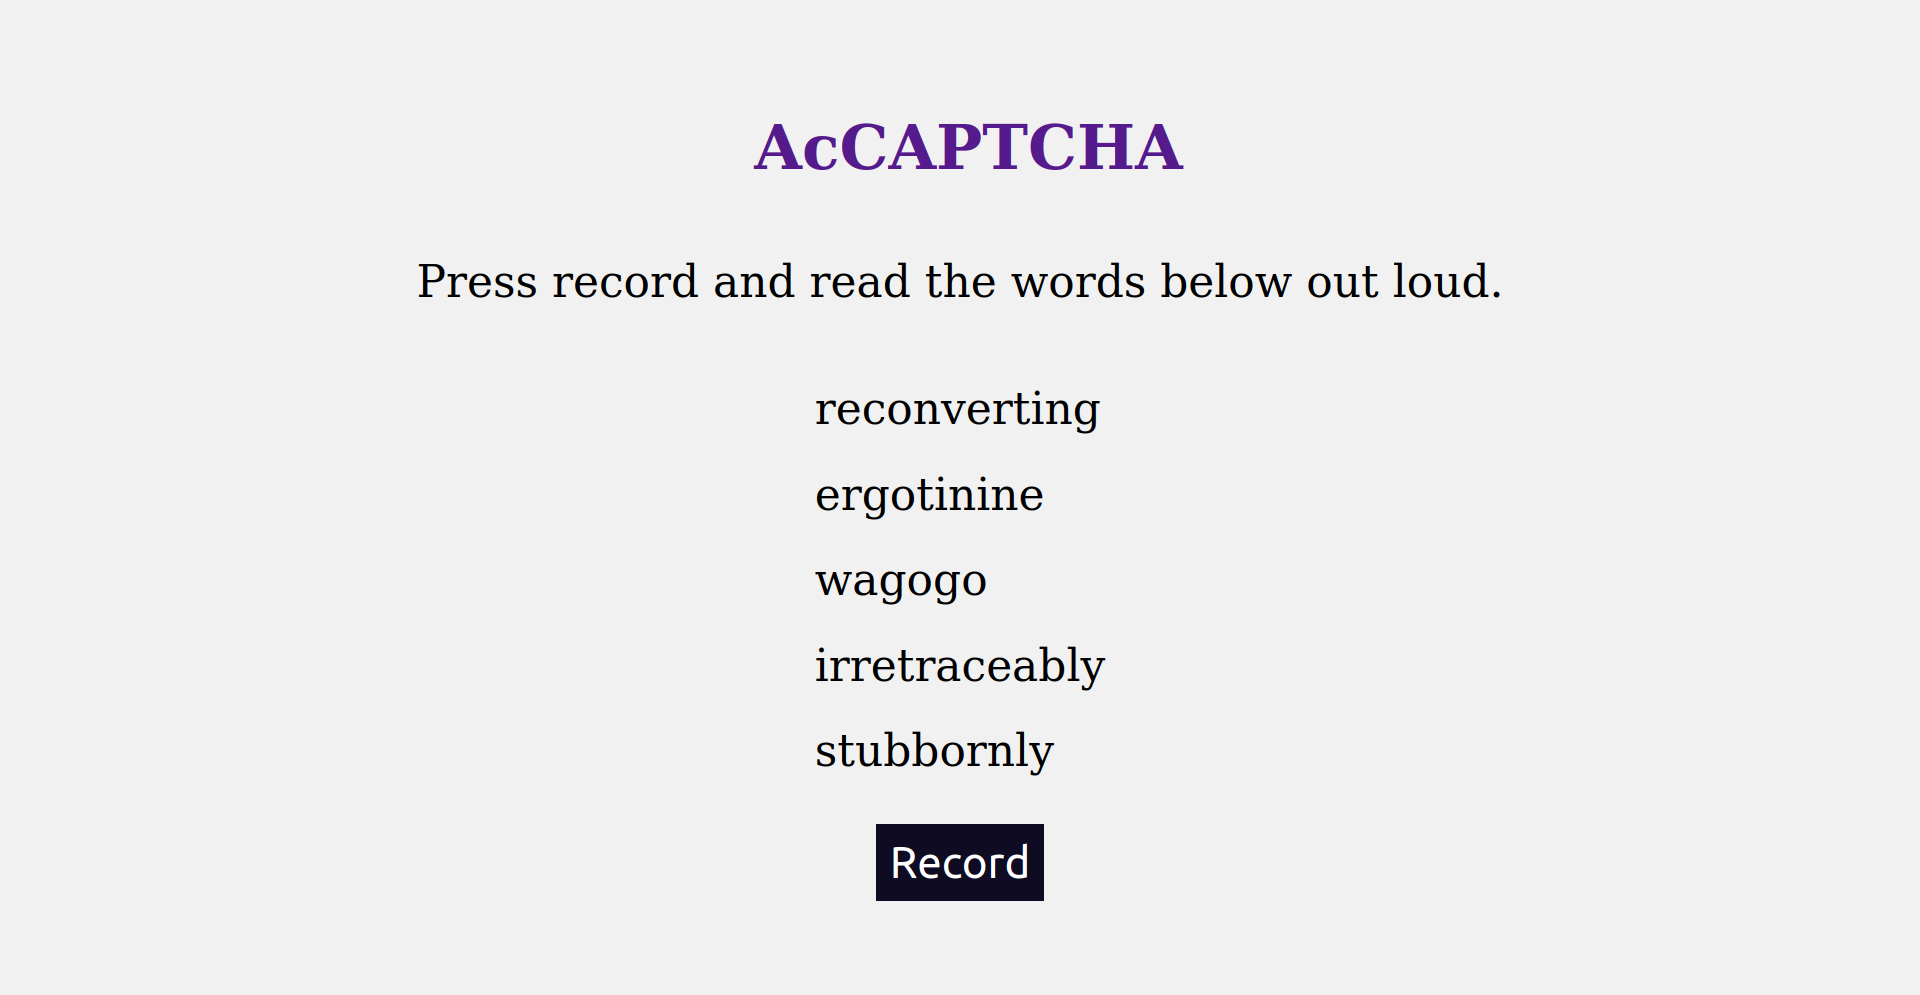
\includegraphics[scale=0.15]{assets/images/word_reading.png}
		\end{figure}
	}

	\begin{itemize}
		\item <2-> Google Cloud Speech API can be openly used with a public API token.
		\item <2-> Slow and does not perform well when dealing with non-english accents.
		\item <2-> Not suitable for non-personal use-cases.
	\end{itemize}


\end{frame}

\begin{frame}
	\frametitle{Configuration}
	\begin{figure}[h!t]
		\centering
		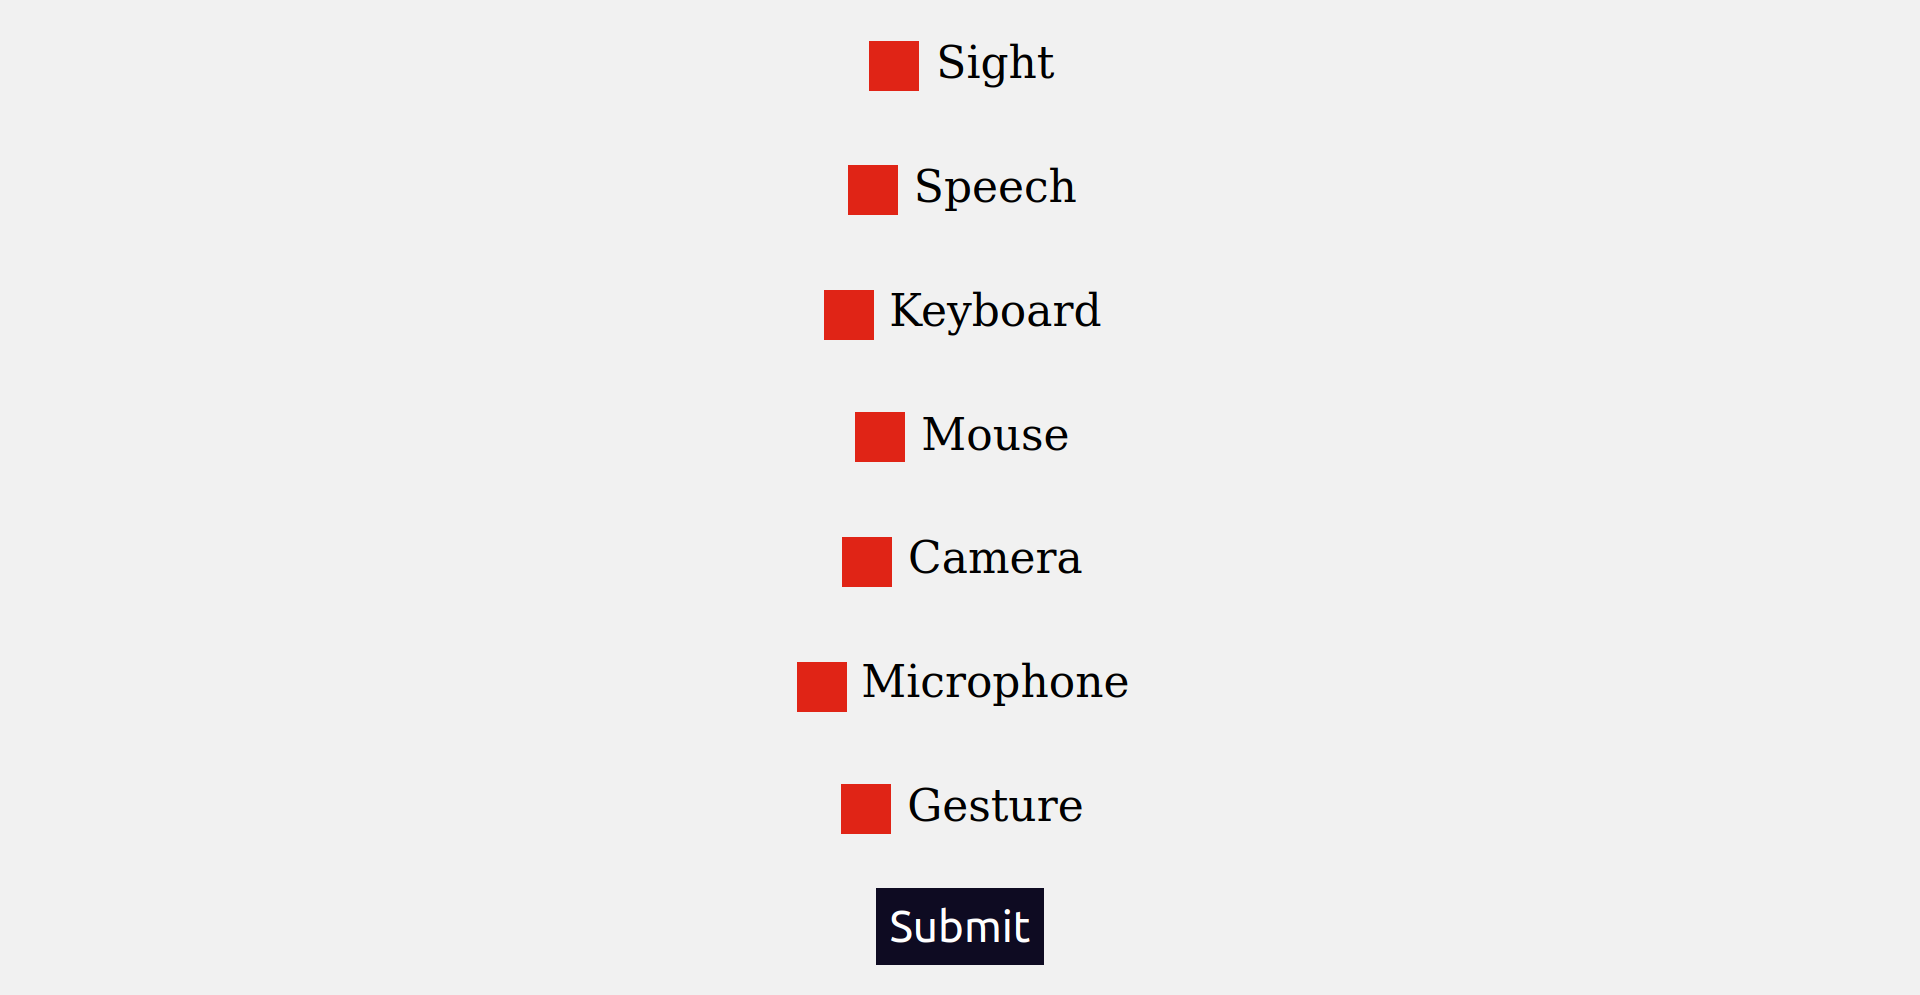
\includegraphics[scale=0.15]{assets/images/configure.png}
	\end{figure}

	\note[item]{By default all chechboxes are unchecked for inclusivity.}
	\note[item]{The proposition we get is a conjuction of flags, if a test is True then it can be sampled.}
\end{frame}

% * Conclusion
\begin{frame}
	\center{
		\huge{
			\textit{
				Thank you
			}
		}
	}
\end{frame}

\end{document}
